%%
%% Copyright (C) 2008  Distributed Computing System (DCS) Group, Computer
%% Science Department - University of Piemonte Orientale, Alessandria (Italy).
%%
%% This program is free software: you can redistribute it and/or modify
%% it under the terms of the GNU Lesser General Public License as published
%% by the Free Software Foundation, either version 3 of the License, or
%% (at your option) any later version.
%%
%% This program is distributed in the hope that it will be useful,
%% but WITHOUT ANY WARRANTY; without even the implied warranty of
%% MERCHANTABILITY or FITNESS FOR A PARTICULAR PURPOSE.  See the
%% GNU Lesser General Public License for more details.
%%
%% You should have received a copy of the GNU Lesser General Public License
%% along with this program.  If not, see <http://www.gnu.org/licenses/>.
%%

\section{Introduzione} \label{sec:intro}

Questa sezione, ha lo scopo di far comprendere all'utente i principi che stanno alla base del funzionamento dell'applicazione \mgTheApp{}; prima di addentrarsi in tale descrizione, verranno forniti alcuni cenni sul ``rendering'' e sul ``Grid computing''.

Nella sezione \S \ref{ssec:intro-render} si illustrano alcune delle problematiche riguardanti il ``rendering'' di immagini e di scene computerizzate; in \S \ref{ssec:intro-grid}, invece, si presenta, brevemente, l'idea che sta alla base del ``Grid computing''; infine, in \S \ref{ssec:intro-theapp} si illustra il funzionamento ad alto livello dell'applicazione \mgTheApp{}.

\subsection{Rendering} \label{ssec:intro-render}

Il \emph{rendering} di immagini o di sequenze di fotogrammi (\emph{frame}) consiste nell'applicare a un modello matematico (tipicamente rappresentato sottoforma di un modello \emph{wire-frame}) una serie di attributi statici o dinamici (come ``texture'', luci, ``bump mapping'', ...) con il fine di ottenere un'immagine o un'animazione completa di dettagli.

Si tratta di un'attivit\`a molto onerosa dal punto di vista computazionale: anche con la tecnologia attuale, il ``rendering'' di animazioni della durata di alcuni minuti pu\`o richiedere diverse ore di computazione, in modo particolare quando tali animazioni includono molti dettagli realistici.

La produzione di animazioni computerizzate e di immagini digitali di elevata qualit\`a, arricchite di dettagli realistici, \`e un'attivit\`a che evolve continuamente, grazie alle innovazioni tecnologiche e ai progressi delle tecniche grafiche.
Mentre, al giorno d'oggi, si \`e in grado di ottenere immagini e animazioni computerizzate che fino a qualche anno fa era impensabile produrre in un tempo relativamente breve, la domanda di potenza computazionale e di capacit\`a di memorizzazione non si \`e arrestata:
\begin{itemize}
\item una maggiore potenza computazionale \`e indispensabile per poter ottenere prodotti grafici di elevata qualit\`a in un tempo sempre pi\`u breve;
\item una maggiore capacit\`a di memorizzazione \`e necessaria in quanto l'aumento della qualit\`a dei dettagli delle immagini ha portato a ottenere prodotti grafici di dimensioni anche dell'ordine dei Gigabyte;
\item una maggiore velocit\`a di accesso ai dispositivi di memorizzazione \`e indispensabile a causa del trasferimento di enormi quantit\`a di dati.
\end{itemize}
Inoltre, mentre le innovazioni tecnologiche permettono la realizzazione di prodotti grafici di qualit\`a superiore, la maggiore accessibilit\`a, da parte degli esperti del settore, a risorse hardware potenti e a software professionali rende il settore della grafica computerizzata sempre pi\`u competitivo:
\begin{itemize}
\item macchine che fino a una decina di anni fa avrebbero richiesto forti investimenti finanziari oggi sono acquistabili a un prezzo relativamente basso;
\item software per la grafica professionale sono ora disponibili a prezzi accessibili o sono addirittura gratuiti.
\end{itemize}
L'applicazione \emph{Blender} \footnote{\href{http://www.blender.org}{http://www.blender.org}} \`e un esempio di software gratuito dotato di funzionalit\`a avanzate, mentre \emph{Elephant Dream} \footnote{\href{http://www.elephantdream.org}{http://www.elephantdream.org}} \`e il primo film di animazione 3D, disponibile gratuitamente, realizzato con un software gratuito come Blender \footnote{Attualmente, altri due film, \emph{Plum\'iferos} (\href{http://www.plumiferos.com}{http://www.plumiferos.com}), rilasciato a breve, e \emph{Peach} (\href{http://peach.blender.org}{http://peach.blender.org}), la cui produzione inizia a Ottobre, utilizzano il software Blender.}.

La soluzione comunemente adottata dai professionisti del settore, per la riduzione dei tempi di produzione, \`e l'utilizzo di un \emph{render-farm} (o \emph{render-wall}), ossia di un gruppo di macchine interconnesse (tipicamente, un ``cluster'') ottimizzate per le operazioni di ``rendering'': i tempi di produzione vengono accorciati attraverso una parallelizzazione del processo di ``rendering'' delle immagini o dei filmati.
In un'articolo apparso sulla rivista \emph{Byte and Switch}, si dice che la \emph{Pixar} avrebbe impiegato pi\`u di $2000$ anni per effettuare il ``rendering'' del film \emph{Cars} se avesse avuto a disposizione un singolo computer, mentre, grazie all'utilizzo di un ``render-farm'', il tutto \`e stato effettuato in soli $5$ anni \cite{ByteAndSwitch2006Pixar}.

L'utilizzo di un ``render-farm'' \`e possibile grazie al fatto che il ``rendering'' di immagini e di animazioni \`e un'attivit\`a altamente parallelizzabile: ogni ``frame'', o gruppo di ``frame'', di un'animazione pu\`o essere processato in modo separato e indipendente dagli altri, inviandolo su una delle macchine del ``render-farm''; in questo modo pi\`u ``frame'' di una stessa animazione possono essere processati contemporaneamente in parallelo su macchine differenti del ``render-farm'', attuando quindi una forma di ``rendering'' pseudo-parallelo. In maniera simile, un'immagine, pu\`o essere scomposta in una serie di mattonelle (\emph{tile}), ognuna delle quali pu\`o essere processata su una differente macchina del ``render-farm''.

Tipicamente, un ``render-farm'' \`e coordinato da un \emph{queue manager} il cui compito principale \`e la gestione dell'accodamento delle immagini e delle animazioni da sottoporre al ``rendering'' e la distribuzione dei relativi ``tile'' o ``frame'' sui computer facenti parte del ``render-farm'', per effettuarne il processamento. Un ``queue-manager'' abbastanza diffuso e disponibile gratuitamente \`e \emph{Dr. Queue} \footnote{\href{http://drqueue.org/cwebsite/}{http://drqueue.org/cwebsite/}}.

Malgrado l'utilizzo di un ``render-farm'' permetta di ridurre drasticamente i tempi di produzione, gli investimenti monetari richiesti per il suo acquisto e la relativa manutenzione sono in generale elevati e non sono sempre accompagnati da un immediato ritorno economico.

\subsection{Grid computing} \label{ssec:intro-grid}

L'avvento del \emph{Grid computing}, come paradigma di computazione, e l'emergere di \emph{sistemi Grid}, che sfruttano tale paradigma, ha reso possibile disporre di una elevata potenza computazionale e una grande capacit\`a di memorizzazione a costi molto ridotti.
L'obiettivo del ``Grid computing'' consiste nel permettere la condivisione, in modo coordinato e distribuito, di risorse eterogenee (tipicamente, computazionali o di memorizzazione) appartenenti a diverse entit\`a (individui o istituzioni), il tutto effettuato in modo trasparente rispetto a chi utilizza un sistema Grid \cite{Foster2001Anatomy}.

Detto in maniera pi\`u semplice, due o pi\`u comunit\`a (singoli utenti, universit\`a, aziende, etc.), anche separate da una larga distanza geografica, possono condividere, attraverso un sistema Grid, le rispettive risorse (di calcolo o di memorizzazione), in modo che gli utenti di ciascuna comunit\`a possano usare, in maniera del tutto trasparente (cio\`e, come se tutto avvenisse sulla propria macchina), le risorse che tutte le comunit\`a hanno messo a disposizione; le comunit\`a quindi hanno a disposizione una potenza computazionale maggiore di quella che avrebbero singolarmente, il tutto con un investimento economico pressoch\'e nullo.

Riguardo le singole propriet\`a di cui, la condivisione ottenuta tramite ``Grid computing'', deve godere, la condivisione distribuita permette, agli utenti del sistema, di utilizzare le varie risorse remote senza preoccuparsi della distanza geografica: le risorse possono essere poste anche a una distanza geografica molto vasta, come, ad esempio, quella su cui la rete Internet si estende.
Il coordinamento delle risorse condivise, invece, \`e necessario per poter interagire con risorse differenti tra loro e, in generale, indipendenti.
La trasparenza, permette agli utenti di un sistema Grid, per esempio, di non preoccuparsi di conoscere la locazione fisica di una certa risorsa (come un file o un programma) o di gestire problematiche derivanti dalla comunicazione di rete all'interno delle proprie applicazioni.

Oltre alle propriet\`a suddette, l'obiettivo del ``Grid computing'' \`e anche di quello di garantire che la condivisione sia sicura (ad es., privatezza, per chi sottomette delle computazioni, e integrit\`a, per chi mette a disposizione le proprie risorse per le computazioni) e che le risorse del sistema siano gestite nel modo pi\`u efficiente possibile.

Il componente di un sistema Grid che si occupa di raggiungere tali obiettivi prende il nome di \emph{middleware}; si tratta di uno strato software che si pone tra il sistema operativo e le applicazioni utente, composto da varie componenti, ognuno dei quali \`e preposto a uno specifico compito (ad es., gestione delle risorse, sicurezza, trasferimento di file, etc.).

Dato che il ``rendering'' di immagini o filmati digitali pu\`o, generalmente, essere scomposto in attivit\`a parallele e indipendenti, \`e possibile sfruttare il ``Grid computing'' per cercare di ridurre i tempi di produzione, in maniera simile a quanto avviene in un ``render-farm''.
I vantaggi che ne derivano comprendono:
\begin{itemize}
\item la riduzione dei tempi di produzione, grazie alla distribuzione del lavoro su diverse macchine;
\item l'abbattimento dei costi, grazie al risparmio sull'acquisto e sulla manutenzione di risorse hardware;
\item una maggiore affidabilit\`a, grazie alla risottomissione del lavoro su altre macchine del sistema, nel caso in cui alcune macchine diventino indisponibili.
\end{itemize}

\subsection{Applicazione \mgTheApp{}} \label{ssec:intro-theapp}

L'obiettivo dell'applicazione \mgTheApp{} \`e quello di sfruttare il ``Grid computing'' per effettuare il ``rendering'' di immagini e di animazioni di grafica computerizzata; attualmente \mgTheApp{} \`e in grado di supportare scene in formato \emph{Blender}.

L'idea di base di \mgTheApp{} \`e simile a quella utilizzata in un ``render-farm'': una scena viene logicamente divisa in gruppi contigui di ``frame'', ognuno dei quali viene processato su una delle macchine del sistema Grid, attualmente disponibili.
Per effettuare l'elaborazione di un certo gruppo di ``frame'' su una particolare macchina del sistema Grid, \mgTheApp{} trasferisce sulle macchine il file della scena insieme a eventuali risorse addizionali (come, ad esempio, delle texture).
Una volta che la computazione sulla macchina remota \`e terminata (ossia, il ``rendering'' di tutti i ``frame'' appartenenti al gruppo \`e stato completato), il risultato viene trasferito sulla macchina locale dell'utente.
Quando tutte le computazioni sono terminate, all'utente non rimane altro che assemblare i risultati ottenuti dal ``rendering'' dei vari gruppi di ``frame''.

Per effettuare tali operazioni, \mgTheApp{} interagisce con lo \emph{scheduler} del sistema Grid, cio\`e con quel componente software che si occupa di selezionare una macchina del sistema Grid e di assegnarle una certa computazione.

Il ruolo principale di \mgTheApp{} \`e, quindi, quello di fornire un'interfaccia ad alto livello tra l'utente, che intende effettuare il ``rendering'' di una scena Blender, e lo ``scheduler'' del sistema Grid. Per effettuare ci\`o, l'utente di \mgTheApp{} deve specificare le seguenti informazioni:
\begin{itemize}
\item \emph{Scene file}, il percorso completo del file della scena (file \mgCode{.blend}, in formato Blender);
\item \emph{Start frame}, il frame iniziale da cui far partire il ``rendering'' dell'intera scena; il valore di default \`e $1$.
\item \emph{End frame}, il frame finale in cui arrestare il ``rendering'' dell'intera scena; il valore di default \`e $1$.
\end{itemize}
L'utente pu\`o inoltre fornire altre informazioni, come:
\begin{itemize}
\item \emph{Scene name}, nome simbolico utilizzato per identificare la scena durante il processo di ``rendering''.
Se non viene specificato, viene costruito a partire dal nome dell'utente (ricavato dal sistema operativo) e dalla data corrente di sistema.
\item \emph{Scene step}, numero massimo di ``frame'' da assegnare a ogni gruppo in cui la scena viene logicamente divisa; pi\`u precisamente, se $F$ \`e il numero di ``frame'' da sottoporre al ``rendering'' e $S$ \`e il valore assunto da ``scene step'', la scena verr\`a logicamente partizionata in $\lceil F/S \rceil$ gruppi di ``frame'' contigui \footnote{L'operatore $\lceil x \rceil$ restituisce l'intero uguale o immediatamente superiore all'argomento $x$, cio\`e restituisce $x$, se $x$ \`e un numero intero, o la parte intera di $x$ incrementata di uno, se $x$ \`un numero reale con parte decimale non nulla.}, ciascuno contenente, al pi\`u, $S$ frame \footnote{Si noti che l'ultimo gruppo, cio\`e quello contenente l'ultimo ``frame'' della scena su cui effettuare il ``rendering'', potrebbe contenere un numero di ``frame'' inferiore a $S$; ci\`o capita quando $F$ non \`e un multiplo di $S$.}.
%L'operatore $\lceil x \rceil$ restituisce l'intero uguale o immediatamente superiore all'argomento $x$, cio\`e restituisce $x$, se $x$ \`e un numero intero, o la parte intera di $x$ incrementata di uno, se $x$ \`un numero reale.
Se tale informazione non viene fornita dall'utente, il valore di default usato da \mgTheApp{} \`e $25$.
\item \emph{Input file}, file, eventualmente compresso in formato ZIP, rappresentante una o pi\`u risorse aggiuntive, come, ad esempio, delle texture.
Se tale informazione non \`e fornita dall'utente, \mgTheApp{} suppone che la scena non abbia bisogno di alcuna risorsa addizionale.
\end{itemize}

La Fig.~\ref{fig:intro-workflow} fornisce una rappresentazione ad alto livello delle varie operazioni eseguite per effettuare il ``rendering'' di una scena tramite \mgTheApp{}.
Il numero che appare accanto alle frecce indica l'ordine temporale secondo cui avvengono le varie azioni:
\begin{enumerate}
\item L'utente crea un modello di una scena di animazione in Blender; in Fig.~\ref{fig:intro-workflow} si suppone che la scena sia composta da $300$ frame.
\item L'utente esegue l'applicazione \mgTheApp{}, inserendo, almeno, le seguenti informazioni:
\begin{itemize}
\item percorso completo al file della scena \mgCode{MyScene.blend};
\item numero del primo ``frame'' da cui far partire il ``rendering'' (in questo caso $1$);
\item numero dell'ultimo ``frame'' in cui far arrestare il ``rendering'' (in questo caso $300$).
\end{itemize}
Nella figura si ipotizza, anche, che l'utente specifichi esplicitamente che come ``step frame'' si utilizzi il valore $100$.
\item Quando l'utente richiede l'esecuzione del ``rendering'', l'applicazione \mgTheApp{}:
\begin{enumerate}
\item suddivide la scena in $300/100=3$ gruppi da $100$ ``frame'' contigui ciascuno: un gruppo per i ``frame'' da $1$ a $100$, uno per i ``frame'' da $101$ a $200$ e, infine, uno per i ``frame'' da $201$ a $300$;
\item contatta lo ``scheduler'' \emph{mygrid} del sistema \emph{ShareGrid};
\item invia allo ``scheduler'' le istruzioni per effettuare il ``rendering'' dei tre gruppi;
\item richiede allo ``scheduler'' l'esecuzione delle tre operazioni di ``rendering''.
\end{enumerate}
\item Lo ``scheduler'' provvede quindi a distribuire le operazioni di ``rendering'' sulle macchine di ShareGrid, non appena diventano disponibili; su ognuna di queste macchina avverr\`a l'effettivo processamento dei ``frame'' tramite Blender.
Occorre far notare che, da questo punto in poi, il ruolo principale di \mgTheApp{} \`e terminato; l'utente pu\`o infatti decidere di:
\begin{itemize} 
\item continuare a usare \mgTheApp{}, per monitorare lo stato di esecuzione del ``rendering'' o per sottomettere un nuovo ``rendering'';
\item usare l'interfaccia (testuale o grafica) dell'applicazione ``mygrid'' per monitorare lo stato di esecuzione del ``rendering'';
\item abbandonare la postazione di lavoro e controllare lo stato di esecuzione saltuariamente \footnote{L'applicazione ``mygrid'' deve per\`o rimanere in esecuzione sulla macchina dell'utente.}.
\end{itemize} 
\item A mano a mano che il ``rendering'' di ogni gruppo di ``frame'' termina, lo ``scheduler'' trasferisce il risultato sulla macchina dell'utente, nella stessa cartella da cui l'applicazione \mgTheApp{} \`e stata eseguita.
Per convenzione, il risultato di un ``rendering'' di un certo gruppo di ``frame'' \`e un file compresso in formato ZIP, il cui nome ha le seguente forma:
\begin{mgCodeBox}
$\langle$nome-file-scena$\rangle$-rendered.zip\_$\langle G_F \rangle$\_$\langle G_L \rangle$
\end{mgCodeBox} 
dove:
\begin{itemize}
\item $\langle$nome-file-scena$\rangle$ \`e il nome del file della scena, escluso il percorso e l'estensione;
\item $\langle G_F \rangle$ \`e il primo ``frame'' del gruppo da cui il ``rendering'' \`e iniziato;
\item $\langle G_L \rangle$ \`e l'ultimo ``frame'' del gruppo in cui il ``rendering'' \`e terminato.
\end{itemize}
Nel caso della figura, i file prodotti dalle tre operazioni di ``rendering'' sono:
\begin{mgCodeBox}
MyScene-rendered.zip\_$1$\_$100$ \newline
MyScene-rendered.zip\_$101$\_$200$ \newline
MyScene-rendered.zip\_$201$\_$300$
\end{mgCodeBox}
All'interno di ogni file compresso, il risultato del ``rendering'' (ad es., file in formato AVI) \`e contenuto dentro una cartella chiamata \emph{$\langle$nome-file-scena$\rangle$-rendered} (nel caso della figura, \emph{MyScene-rendered}).
\item Quando i ``rendering'' dei tre gruppi sono tutti terminati, l'utente pu\`o combinare in modo opportuno il contenuto dei tre file compressi.
\end{enumerate}

\begin{figure}
\centering
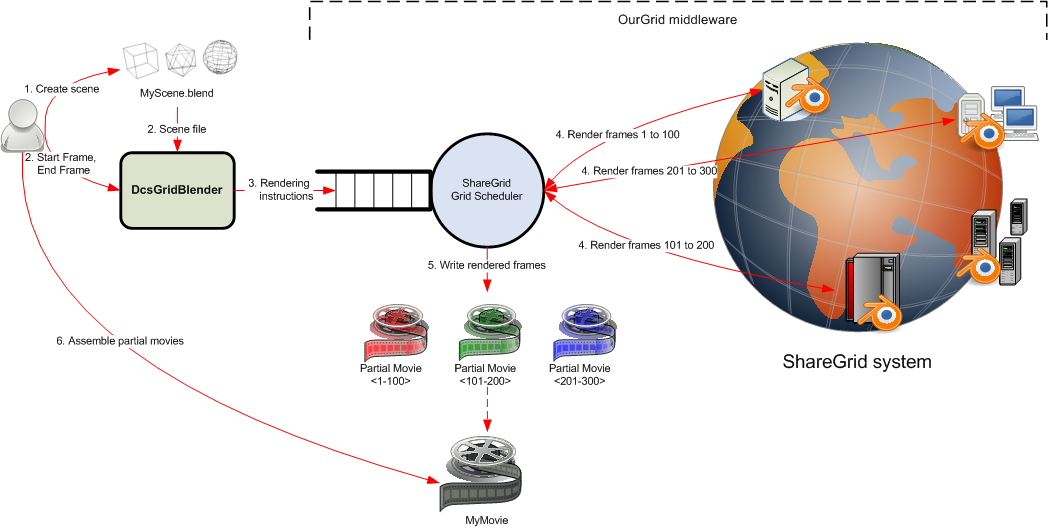
\includegraphics[scale=0.40]{images/DcsShareGridBlender_Block}
\caption{Workflow per il rendering di una scena tramite \mgTheApp{}.}
\label{fig:intro-workflow}
\end{figure}
